\section{Results}
\label{sec:results}

\subsection{Benchmark Comparison}
\label{subsec:benchmark}

Table~\ref{tab:benchmark} reports the region-based segmentation performance of every evaluated model on the held-out test subsets of ISIC 2016, ISIC 2017, and ISIC 2018 --- the four baseline networks (U-Net, Attention U-Net, UNet++, and TransUNet), the MAFF-Net~\cite{ref15} architecture reproduced under this study's protocol as a prior-work reference control, and the SpecGate-Net introduced in this work. The reproduction is neither a proposed model nor an external baseline; it situates the SpecGate-Net against a faithful account of the prior architecture. The Dice coefficient and the IoU are the principal indicators, with accuracy, sensitivity, and specificity reported alongside.

\begin{table*}[!t]
\centering
\caption{Region-based segmentation performance on the held-out test subsets of
ISIC 2016, ISIC 2017, and ISIC 2018. Each dataset block lists four external baselines (U-Net, Attention U-Net, UNet++, TransUNet), the MAFF-Net~\cite{ref15} architecture reproduced under this study's protocol as a prior-work reference control, and the SpecGate-Net introduced in this work. The highest value in each column, within each dataset, is shown in bold. The MAFF-Net~\cite{ref15} rows report a reproduction of the published architecture trained and evaluated under the protocol of this study, not the results reported in~\cite{ref15}.}
\label{tab:benchmark}
\setlength{\tabcolsep}{5pt}
\footnotesize
\begin{tabular}{llccccc}
\toprule
Dataset & Method & Dice & IoU & Accuracy & Sensitivity & Specificity \\
\midrule
\multirow{6}{*}{ISIC 2016}
 & U-Net & 0.7874 & 0.6808 & 0.8951 & 0.7649 & 0.9609 \\
 & Attention U-Net & 0.8466 & 0.7443 & 0.9178 & 0.8780 & 0.9495 \\
 & UNet++ & 0.8141 & 0.7140 & 0.9055 & 0.7996 & 0.9647 \\
 & TransUNet & 0.8365 & 0.7349 & 0.9161 & 0.8077 & \textbf{0.9700} \\
 & MAFF-Net~\cite{ref15} & \textbf{0.9183} & \textbf{0.8555} & 0.9541 & \textbf{0.9414} & 0.9545 \\
 & SpecGate-Net & 0.9169 & 0.8517 & \textbf{0.9548} & 0.9220 & 0.9689 \\
\midrule
\multirow{6}{*}{ISIC 2017}
 & U-Net & 0.7229 & 0.6152 & 0.9031 & 0.7211 & 0.9562 \\
 & Attention U-Net & 0.8097 & 0.7159 & 0.9331 & 0.8223 & 0.9737 \\
 & UNet++ & 0.7884 & 0.6959 & 0.9291 & 0.7776 & 0.9784 \\
 & TransUNet & 0.8683 & 0.7843 & 0.9561 & 0.8418 & \textbf{0.9870} \\
 & MAFF-Net~\cite{ref15} & \textbf{0.9116} & \textbf{0.8447} & \textbf{0.9700} & \textbf{0.9171} & 0.9807 \\
 & SpecGate-Net & 0.9096 & 0.8421 & 0.9682 & 0.9069 & 0.9842 \\
\midrule
\multirow{6}{*}{ISIC 2018}
 & U-Net & 0.6866 & 0.5714 & 0.8732 & 0.7766 & 0.8948 \\
 & Attention U-Net & 0.7662 & 0.6641 & 0.9207 & 0.8352 & 0.9497 \\
 & UNet++ & 0.6978 & 0.5878 & 0.8912 & 0.7692 & 0.9298 \\
 & TransUNet & 0.8259 & 0.7265 & 0.9259 & 0.8929 & 0.9315 \\
 & MAFF-Net~\cite{ref15} & \textbf{0.8844} & \textbf{0.8080} & \textbf{0.9584} & \textbf{0.8973} & 0.9730 \\
 & SpecGate-Net & 0.8701 & 0.7900 & 0.9493 & 0.8733 & \textbf{0.9768} \\
\bottomrule
\end{tabular}
\end{table*}

Among the baselines, the U-Net records the lowest Dice coefficient on all three datasets --- 0.7874, 0.7229, and 0.6866 on ISIC 2016, ISIC 2017, and ISIC 2018 --- with IoU values of 0.6808, 0.6152, and 0.5714. The ordering of the remaining baselines is not constant: on ISIC 2016 the Attention U-Net attains the highest baseline Dice coefficient, 0.8466, ahead of the TransUNet at 0.8365 and the UNet++ at 0.8141, whereas on ISIC 2017 and ISIC 2018 the TransUNet leads, at 0.8683 and 0.8259, followed by the Attention U-Net at 0.8097 and 0.7662 and the UNet++ at 0.7884 and 0.6978. The TransUNet is therefore the strongest baseline on two datasets and the Attention U-Net on the third.

The SpecGate-Net and the MAFF-Net~\cite{ref15} reproduction both record higher Dice and IoU values than every baseline on every dataset. Relative to the strongest baseline on each dataset, the SpecGate-Net records higher Dice coefficients by 0.0703, 0.0413, and 0.0442 on ISIC 2016, 2017, and 2018.

Between the SpecGate-Net and the MAFF-Net~\cite{ref15}, the ordering is consistent across all three datasets. The MAFF-Net~\cite{ref15} records the highest Dice coefficient and IoU of all evaluated models --- Dice 0.9183, 0.9116, and 0.8844 and IoU 0.8555, 0.8447, and 0.8080 on ISIC 2016, 2017, and 2018 --- and the SpecGate-Net records the second-highest, with Dice 0.9169, 0.9096, and 0.8701 and IoU 0.8517, 0.8421, and 0.7900. The Dice differences between the MAFF-Net~\cite{ref15} and the SpecGate-Net are 0.0014, 0.0020, and 0.0143 on the three datasets.

The remaining measures do not always follow the Dice ordering. The SpecGate-Net attains the highest accuracy of all models on ISIC 2016, 0.9548 against 0.9541 for the MAFF-Net~\cite{ref15}, whereas the MAFF-Net~\cite{ref15} leads on ISIC 2017 and ISIC 2018, at 0.9700 and 0.9584. For specificity, the SpecGate-Net exceeds the MAFF-Net~\cite{ref15} on all three datasets --- 0.9689 against 0.9545, 0.9842 against 0.9807, and 0.9768 against 0.9730 --- the last being the highest specificity on ISIC 2018, though the TransUNet attains the highest specificity of all models on ISIC 2016 and ISIC 2017, at 0.9700 and 0.9870. For sensitivity, the MAFF-Net~\cite{ref15} exceeds the SpecGate-Net on all three datasets, at 0.9414, 0.9171, and 0.8973; on ISIC 2018 the TransUNet's 0.8929 exceeds the SpecGate-Net at 0.8733.

A consistent trend spans the three benchmarks: every model records its lowest Dice and IoU on ISIC 2018, and every model except the TransUNet its highest on ISIC 2016 (the TransUNet peaks on ISIC 2017). The spread between the strongest and weakest models is also widest on ISIC 2018, where Dice coefficients range from 0.6866 to 0.8844, against 0.7874 to 0.9183 on ISIC 2016. Each value corresponds to a single training run per configuration, so the narrower differences between models should be interpreted with corresponding caution.

\subsection{Boundary Evaluation}
\label{subsec:boundeval}

In dermoscopic segmentation the practical value of a prediction depends heavily on the fidelity of the lesion margin, since the margin determines the measured extent of the lesion and is where annotation and prediction most often diverge. The region-overlap measures reported above, however, are dominated by the comparatively large and homogeneous interior: a contour displaced by a few pixels alters the overlap only marginally, so a model may attain a high overlap score while reproducing the margin imprecisely. Measures defined directly on the contour are therefore required. Table~\ref{tab:boundary} reports the three boundary-based measures of Section~\ref{subsec:metrics} --- the 95th-percentile Hausdorff distance, the average symmetric surface distance, and the Boundary IoU --- for every model on the three datasets.

\begin{table*}[!t]
\centering
\caption{Boundary-based segmentation performance on the held-out test subsets of
ISIC 2016, ISIC 2017, and ISIC 2018. HD95 and ASSD are expressed in pixels of
the $384\times384$ evaluation grid, and lower values indicate closer agreement;
higher Boundary IoU values indicate closer agreement. Rows are grouped as in Table~\ref{tab:benchmark}: four external baselines, the MAFF-Net~\cite{ref15} architecture reproduced under this study's protocol as a reference control, and the SpecGate-Net. The column
$n_{\mathrm{valid}}$ gives the number of images contributing to the distance
measures. The best value in each column, within each dataset, is shown in bold. The MAFF-Net~\cite{ref15} rows report a reproduction of the published architecture trained and evaluated under the protocol of this study, not the results reported in~\cite{ref15}.}
\label{tab:boundary}
\setlength{\tabcolsep}{6pt}
\footnotesize
\begin{tabular}{llcccc}
\toprule
Dataset & Method & HD95 (px) & ASSD (px) & Boundary IoU & $n_{\mathrm{valid}}/n$ \\
\midrule
\multirow{6}{*}{ISIC 2016}
 & U-Net & 61.976 & 22.527 & 0.3195 & 192 / 192 \\
 & Attention U-Net & 50.465 & 18.221 & 0.2436 & 192 / 192 \\
 & UNet++ & 48.244 & 18.341 & 0.3283 & 190 / 192 \\
 & TransUNet & 43.779 & 16.368 & 0.2898 & 192 / 192 \\
 & MAFF-Net~\cite{ref15} & \textbf{21.979} & \textbf{8.336} & \textbf{0.4518} & 192 / 192 \\
 & SpecGate-Net & 23.329 & 8.510 & 0.4514 & 192 / 192 \\
\midrule
\multirow{6}{*}{ISIC 2017}
 & U-Net & 60.572 & 23.027 & 0.3560 & 194 / 200 \\
 & Attention U-Net & 40.745 & 17.004 & 0.3749 & 198 / 200 \\
 & UNet++ & 42.561 & 15.603 & 0.4244 & 197 / 200 \\
 & TransUNet & 26.750 & 9.710 & 0.4585 & 200 / 200 \\
 & MAFF-Net~\cite{ref15} & \textbf{16.788} & \textbf{6.565} & 0.5255 & 200 / 200 \\
 & SpecGate-Net & 16.869 & 6.645 & \textbf{0.5277} & 200 / 200 \\
\midrule
\multirow{6}{*}{ISIC 2018}
 & U-Net & 72.867 & 29.454 & 0.2958 & 388 / 392 \\
 & Attention U-Net & 47.746 & 19.645 & 0.3035 & 385 / 392 \\
 & UNet++ & 63.710 & 25.348 & 0.2672 & 383 / 392 \\
 & TransUNet & 41.836 & 15.092 & 0.3406 & 392 / 392 \\
 & MAFF-Net~\cite{ref15} & \textbf{20.570} & \textbf{8.199} & \textbf{0.4701} & 392 / 392 \\
 & SpecGate-Net & 22.554 & 9.240 & 0.4611 & 391 / 392 \\
\bottomrule
\end{tabular}
\end{table*}

The distance measures are undefined when a prediction contains no positive pixels; the affected images are excluded from the means and accounted for in the column $n_{\mathrm{valid}}$. Such cases arise for only a minority of images, predominantly among the baselines: the UNet++ produces an empty prediction for nine images of ISIC 2018 and the Attention U-Net for seven, whereas the TransUNet and the MAFF-Net~\cite{ref15} produce none on any dataset and the SpecGate-Net produces one, on ISIC 2018. The Boundary IoU is defined for all images and computed over the complete test subsets.

The SpecGate-Net and the MAFF-Net~\cite{ref15} reproduction both record lower HD95, lower ASSD, and higher Boundary IoU than every baseline on each of the three datasets --- the separation holding for all three measures simultaneously and on every dataset, not for an isolated measure or benchmark. Against the strongest baseline for each measure, the SpecGate-Net reduces the HD95 from 43.779 to 23.329 pixels on ISIC 2016, from 26.750 to 16.869 on ISIC 2017, and from 41.836 to 22.554 on ISIC 2018, and the ASSD from 16.368 to 8.510, from 9.710 to 6.645, and from 15.092 to 9.240 pixels on the same datasets. Its Boundary IoU exceeds the highest baseline value by 0.1231, 0.0692, and 0.1205 on ISIC 2016, 2017, and 2018.

Between the SpecGate-Net and the MAFF-Net~\cite{ref15}, the MAFF-Net~\cite{ref15} records the lower HD95 and ASSD on all three datasets --- 21.979 and 8.336 pixels on ISIC 2016, 16.788 and 6.565 on ISIC 2017, and 20.570 and 8.199 on ISIC 2018 --- against 23.329 and 8.510, 16.869 and 6.645, and 22.554 and 9.240 pixels for the SpecGate-Net. For the Boundary IoU the ordering is not uniform: the SpecGate-Net records the highest value of all models on ISIC 2017, 0.5277 against 0.5255, while the MAFF-Net~\cite{ref15} is higher on ISIC 2016, 0.4518 against 0.4514, and ISIC 2018, 0.4701 against 0.4611.

The orderings induced by the boundary measures do not coincide with those from region overlap, indicating that region overlap alone does not fully characterise contour quality. On ISIC 2016 the Attention U-Net records the highest Dice coefficient among the baselines yet the lowest Boundary IoU of all models, 0.2436, below the 0.3195 of the U-Net, which has the lowest Dice on that dataset. A comparable disagreement occurs on ISIC 2018, where the UNet++ records a higher Dice than the U-Net, 0.6978 against 0.6866, but a lower Boundary IoU, 0.2672 against 0.2958. Two models may therefore attain similar region overlap while differing appreciably in contour agreement, so the boundary measures provide information the region measures do not.

Three qualifications apply to the values in Table~\ref{tab:boundary}. Each corresponds to a single training run; the paired significance tests of Section~\ref{subsec:statsig} treat images as the unit of analysis and therefore do not establish differences across training runs, so the differences between closely ranked models, in particular between the SpecGate-Net and the MAFF-Net~\cite{ref15}, should be regarded as observations on these runs rather than as effects established across runs. The per-image dispersion is moreover large relative to the differences between neighbouring models: the standard deviation of the HD95 is of the same order as its mean for every model, ranging from 21.7 to 30.3 pixels for the SpecGate-Net and the MAFF-Net~\cite{ref15} and from 33.9 to 64.8 pixels for the baselines. Finally, as noted in Section~\ref{subsec:metrics}, HD95 and ASSD are in pixels of the 384$\times$384 grid rather than physical units, so they are comparable among the models here but not with distances reported in millimetres elsewhere.

\subsection{Statistical Significance}
\label{subsec:statsig}

The per-image analysis described in Section~\ref{subsec:stats} tests whether the differences summarised in Tables~\ref{tab:benchmark} and~\ref{tab:boundary} are statistically discernible rather than incidental. For every dataset and every metric the Friedman test rejects the hypothesis that the six models are equivalent (all $p<10^{-38}$). The post-hoc comparisons separate the SpecGate-Net from the four baselines cleanly: on all five metrics and all three datasets it exceeds every baseline by a Holm-adjusted margin significant at $\alpha=0.05$ (all $p_{\mathrm{Holm}}\le 1.4\times10^{-10}$), with large effect sizes (matched-pairs rank-biserial $\lvert r\rvert\ge 0.53$). The advantage of the boundary-oriented design over the standard baselines is therefore statistically supported on both the region-based and the boundary-based measures, rather than being an artefact of aggregate averaging.

\begin{table*}[!t]
\centering
\caption{Paired statistical comparison of the SpecGate-Net against the MAFF-Net~\cite{ref15} reproduction, by dataset and metric, on the held-out test images. Across all six models the Friedman omnibus test rejects equality for every dataset and metric (all $p<10^{-38}$). Each entry gives the median paired difference $\Delta$ (SpecGate-Net $-$ MAFF-Net~\cite{ref15}), the matched-pairs rank-biserial effect size $r$, and the Holm-adjusted post-hoc Wilcoxon signed-rank $p$-value ($^{*}$: significant at $\alpha=0.05$). A positive $\Delta$ favours the SpecGate-Net for Dice, IoU, and
Boundary IoU, and favours the MAFF-Net~\cite{ref15} for HD95 and ASSD, which are
error measures. HD95 and ASSD use complete-case pairing over the images for
which both models produced a non-empty prediction. The four baselines are
omitted here: the SpecGate-Net exceeds every baseline on every metric and dataset (all $p_{\mathrm{Holm}}\le 1.4\times10^{-10}$, $\lvert r\rvert\ge 0.53$).}
\label{tab:stats}
\setlength{\tabcolsep}{6pt}
\footnotesize
\begin{tabular}{llccc}
\toprule
 & & \multicolumn{3}{c}{vs.\ MAFF-Net~\cite{ref15}} \\
\cmidrule(lr){3-5}
Dataset & Metric & median $\Delta$ & $r$ & $p_{\mathrm{Holm}}$ \\
\midrule
\multirow{5}{*}{ISIC 2016}
 & Dice  & $+0.0009$ & $0.00$  & $0.962$ \\
 & IoU   & $+0.0017$ & $0.00$  & $0.968$ \\
 & HD95  & $-0.0598$ & $-0.02$ & $0.789$ \\
 & ASSD  & $-0.1204$ & $-0.03$ & $0.721$ \\
 & B-IoU & $+0.0100$ & $+0.08$ & $0.357$ \\
\midrule
\multirow{5}{*}{ISIC 2017}
 & Dice  & $+0.0007$ & $+0.05$ & $0.580$ \\
 & IoU   & $+0.0011$ & $+0.05$ & $0.550$ \\
 & HD95  & $-0.0711$ & $+0.04$ & $0.631$ \\
 & ASSD  & $-0.0465$ & $-0.04$ & $0.613$ \\
 & B-IoU & $+0.0055$ & $+0.10$ & $0.238$ \\
\midrule
\multirow{5}{*}{ISIC 2018}
 & Dice  & $-0.0029$ & $-0.14$ & $0.015^{*}$        \\
 & IoU   & $-0.0053$ & $-0.14$ & $0.017^{*}$        \\
 & HD95  & $+0.4843$ & $+0.23$ & $<\!10^{-3}\,^{*}$ \\
 & ASSD  & $+0.1473$ & $+0.16$ & $0.006^{*}$        \\
 & B-IoU & $-0.0104$ & $-0.10$ & $0.089$            \\
\bottomrule
\end{tabular}
\end{table*}

The comparison with the MAFF-Net~\cite{ref15} reproduction is more nuanced and is reported in Table~\ref{tab:stats}. Against the MAFF-Net~\cite{ref15} the SpecGate-Net is not found to be superior on any dataset: the two are statistically indistinguishable on ISIC 2016 and ISIC 2017 across all five metrics ($p_{\mathrm{Holm}}\ge 0.23$, $\lvert r\rvert\le 0.10$), and on ISIC 2018 the four significant differences all favour the MAFF-Net~\cite{ref15} --- higher Dice and IoU and lower HD95 and ASSD --- with small effect sizes ($\lvert r\rvert\le 0.23$), while the Boundary IoU difference is not significant. The statistical analysis therefore reinforces rather than overturns the positioning adopted throughout this paper: the SpecGate-Net is not established as an improvement over the MAFF-Net~\cite{ref15}, which remains at least its equal and is significantly closer to the reference contours on the largest benchmark.

These conclusions concern the dispersion across test images within a single training run; as set out in Section~\ref{subsec:limitations}, they do not address the variability between training runs, for which repetition across several seeds would be required.

\subsection{Architecture Ablation}
\label{subsec:ablationr}

The three components introduced in this work --- the Frequency Branch, the Feature Alignment Module, and the Gated Fusion Module --- were examined by the leave-one-out ablation of Section~\ref{subsec:protocol}, in which each is disabled in turn while the rest of the network and the training configuration are held fixed. The study was conducted on ISIC 2018. Table~\ref{tab:ablation} reports both the region-based and boundary-based measures for the complete model and the three ablated configurations, so that the two families may be considered together.

\begin{table*}[!t]
\centering
\caption{Leave-one-out architecture ablation of the SpecGate-Net on the ISIC 2018 test subset. HD95
and ASSD are expressed in pixels of the $384\times384$ evaluation grid, and lower
values indicate closer agreement; higher Dice, IoU, accuracy, and Boundary IoU
values indicate closer agreement. The best value in each column is shown in
bold.}
\label{tab:ablation}
\setlength{\tabcolsep}{6pt}
\small
\begin{tabular}{lcccccc}
\toprule
Configuration & Dice & IoU & Accuracy & HD95 (px) & ASSD (px) & Boundary IoU \\
\midrule
Full SpecGate-Net & 0.8701 & 0.7900 & 0.9493 & \textbf{22.554} & \textbf{9.240} & \textbf{0.4611} \\
without Frequency Branch & 0.8708 & 0.7868 & 0.9496 & 23.574 & 9.546 & 0.4416 \\
without Feature Alignment Module & 0.8649 & 0.7811 & 0.9502 & 23.676 & 9.869 & 0.4326 \\
without Gated Fusion Module & \textbf{0.8725} & \textbf{0.7907} & \textbf{0.9520} & 25.546 & 9.488 & 0.4508 \\
\bottomrule
\end{tabular}
\end{table*}

On the boundary-based measures, the complete SpecGate-Net records the best value of the four configurations on all three: the lowest HD95 at 22.554 pixels, the lowest ASSD at 9.240 pixels, and the highest Boundary IoU at 0.4611. Disabling any one component degrades all three simultaneously: removing the Frequency Branch increases the HD95 by 1.020 pixels and the ASSD by 0.306 and reduces the Boundary IoU by 0.0195; removing the Feature Alignment Module increases them by 1.122 and 0.629 pixels and reduces the Boundary IoU by 0.0285; and removing the Gated Fusion Module increases them by 2.992 and 0.248 pixels and reduces the Boundary IoU by 0.0103. No single component accounts for the whole difference, and the ordering depends on the measure: the largest HD95 increase follows removal of the Gated Fusion Module, the largest ASSD increase and Boundary IoU reduction that of the Feature Alignment Module.

The region-based measures do not separate the four configurations in the same way, and do not favour the complete model. The Dice coefficient varies from 0.8649 to 0.8725, a spread of 0.0076, and the complete model, at 0.8701, does not record the highest value: the configuration without the Gated Fusion Module records the highest Dice at 0.8725, IoU at 0.7907, and accuracy at 0.9520, while the complete model records the lowest accuracy of the four, 0.9493. The only configuration whose Dice falls below the complete model's is the one without the Feature Alignment Module, at 0.8649. The present evidence therefore does not support the proposition that these components improve region overlap, and no such claim is made.

Considered together, the two families indicate that the effect of the three components is confined to the fidelity of the predicted contour rather than the extent of the predicted region. This is consistent with Section~\ref{subsec:boundeval}, that region overlap is comparatively insensitive to contour displacements: a configuration may reproduce the lesion area to within a small Dice difference while agreeing less closely with the reference contour. On this evidence, the architectural contribution of the present work is accordingly an improvement in boundary fidelity, not in region-overlap performance.

Three qualifications delimit these observations. Each configuration was trained once, with a single experimental seed, and no repeated runs or statistical testing were performed; the differences in Table~\ref{tab:ablation} are therefore observations on these particular runs, not established as statistically significant. The magnitudes are moreover small relative to the per-image dispersion noted in Section~\ref{subsec:boundeval}, which further limits the weight individual differences can bear. Finally, the study was conducted on ISIC 2018 alone, so the consistency of these observations across the other two datasets is not established here.

\subsection{Qualitative Analysis}
\label{subsec:qual}

\begin{figure*}[t]
\centering
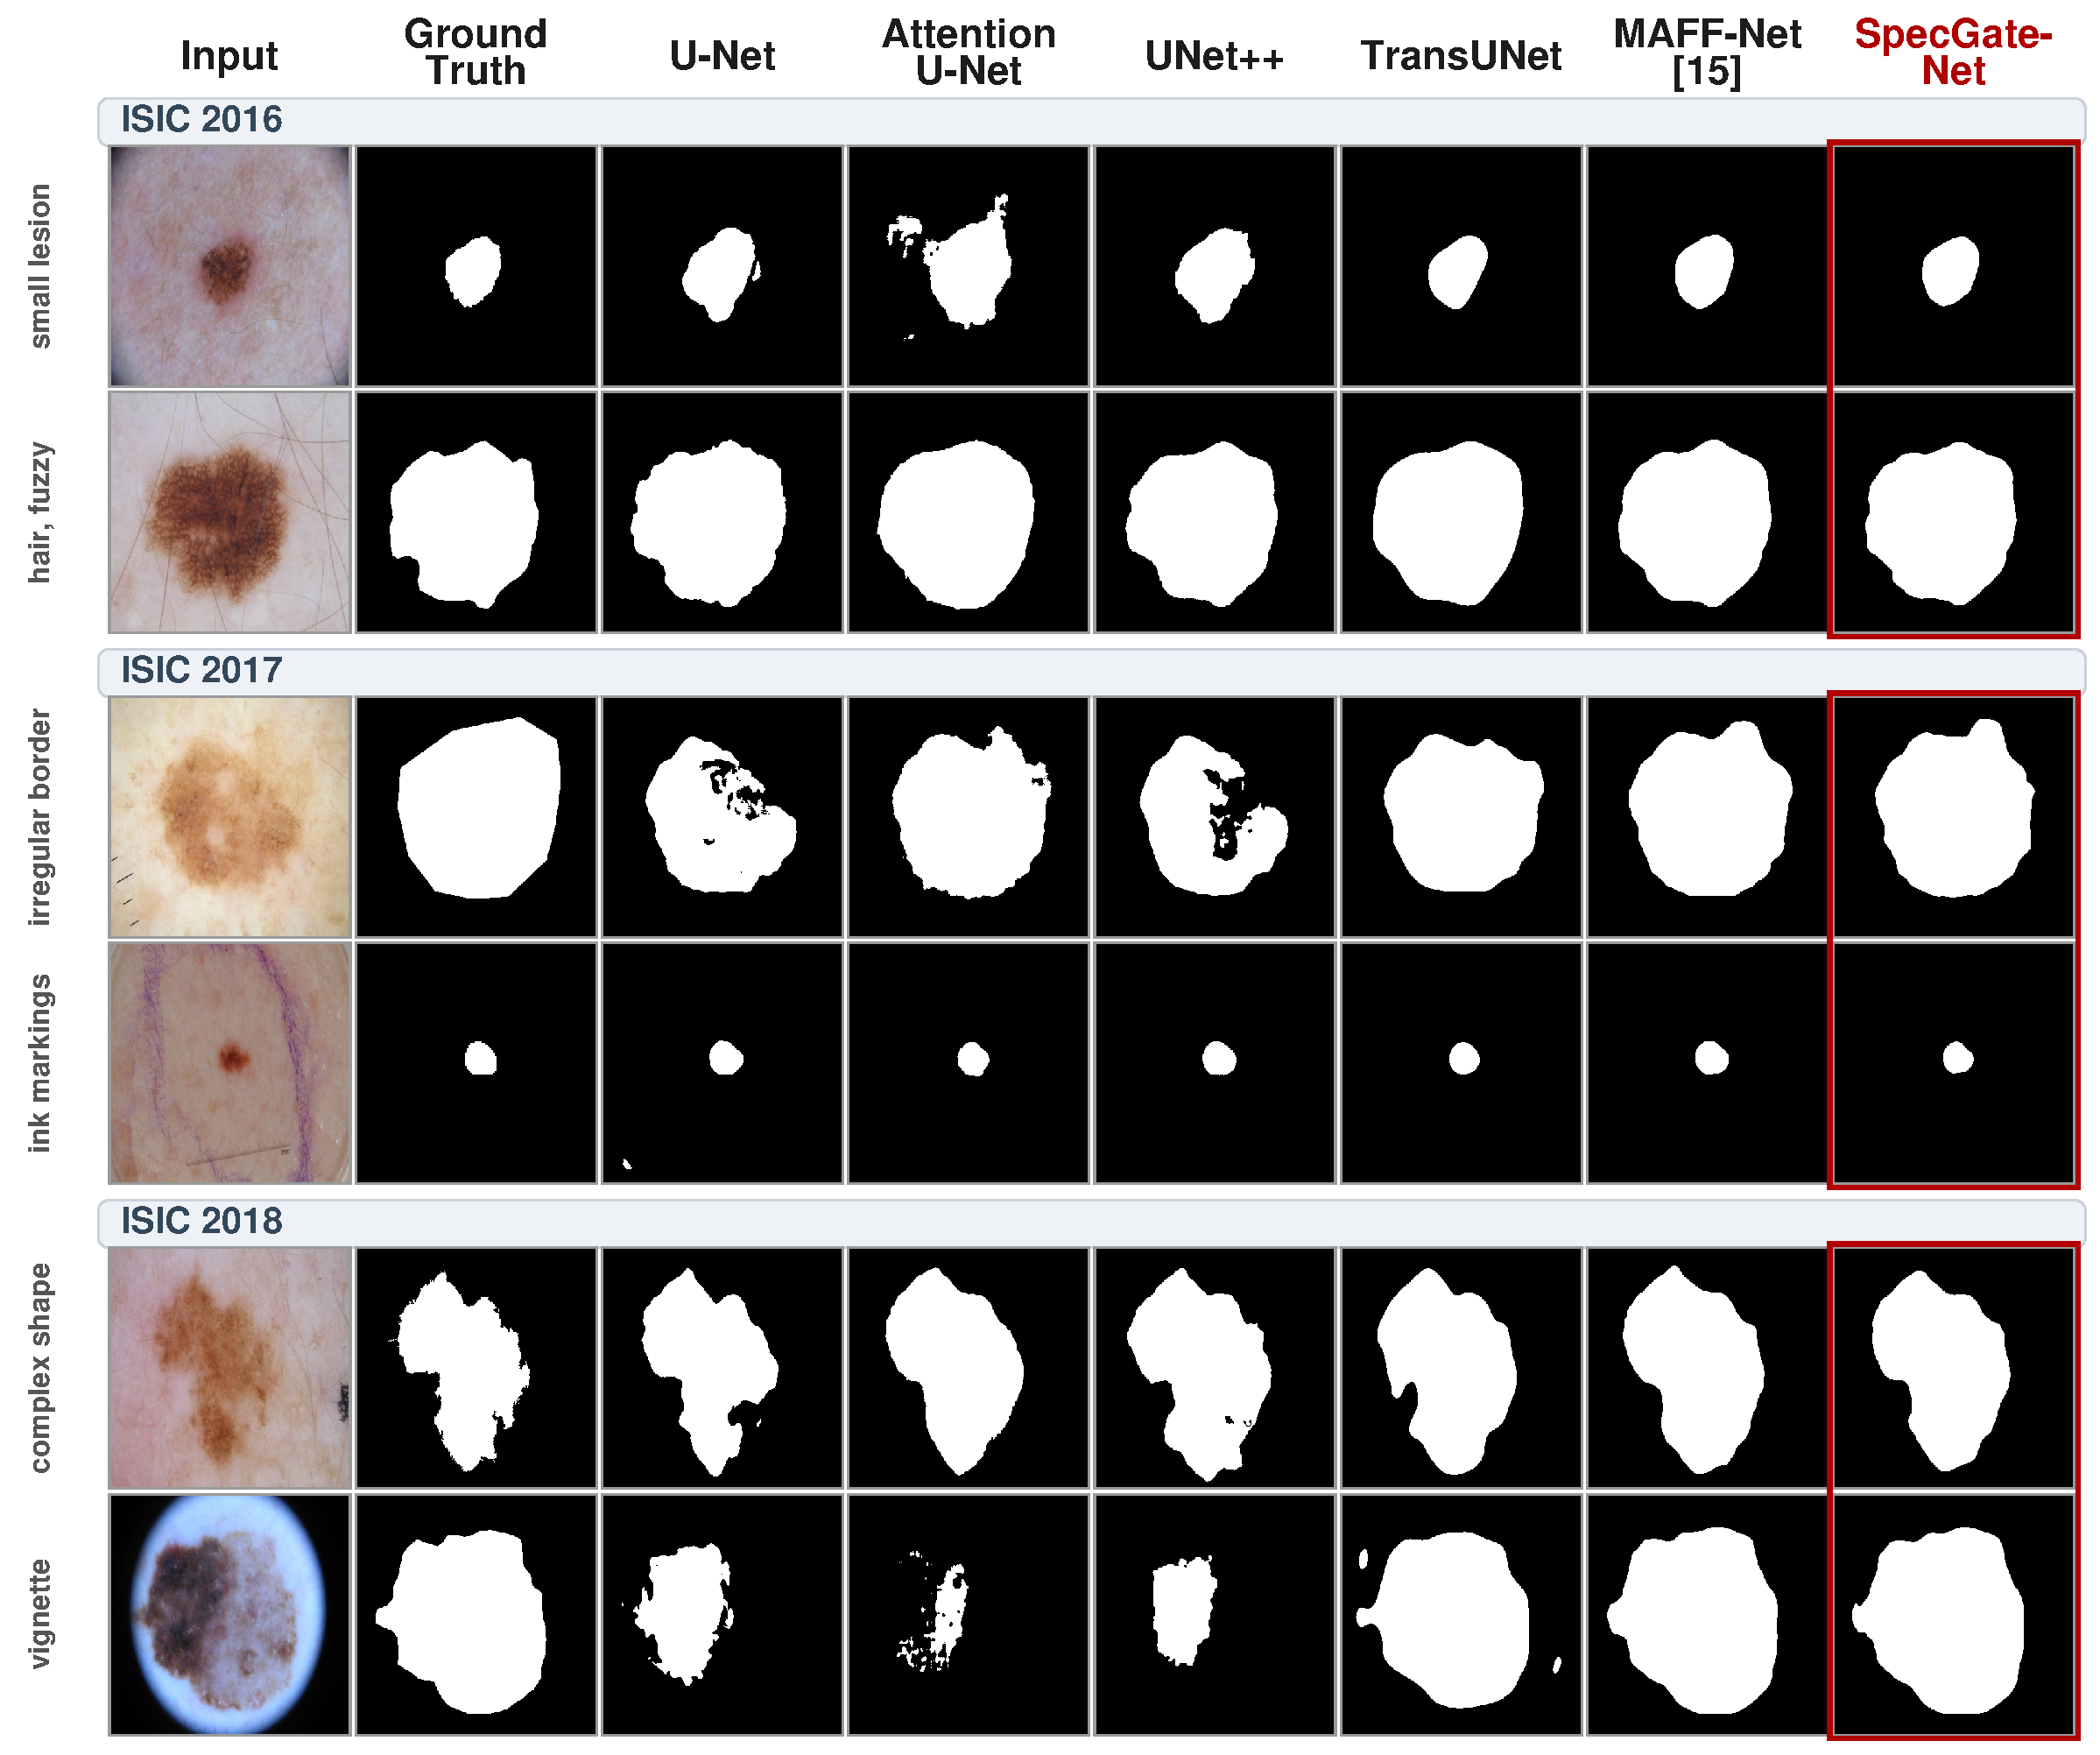
\includegraphics[width=\textwidth]{Figure4_MultiDataset.pdf}
\caption{Qualitative comparison across the ISIC 2016, 2017, and 2018 benchmarks.
Each row shows one challenging lesion --- the input image and ground-truth mask
with the predictions of six models: the four baselines (U-Net, Attention U-Net,
UNet++, TransUNet), the MAFF-Net~\cite{ref15}, and the SpecGate-Net (outlined). Predictions are
unprocessed; examples are from the validation split, whereas
Tables~\ref{tab:benchmark}--\ref{tab:ablation} use the held-out test split. Here MAFF-Net~\cite{ref15} denotes that reproduction rather than the results reported in~\cite{ref15}.}
\label{fig:qualitative}
\end{figure*}

The quantitative measures above summarise agreement over entire test subsets and do not reveal how the predicted contours depart from the reference annotations. Fig.~\ref{fig:qualitative} accordingly presents representative qualitative examples from the ISIC 2016, ISIC 2017, and ISIC 2018 benchmarks, each row showing the same input image and ground-truth mask together with the predictions of the four baselines, the MAFF-Net~\cite{ref15}, and the SpecGate-Net. The cases are selected to span difficulties characteristic of dermoscopic imaging --- small and low-contrast lesions, hair occlusion, irregular shape, ink markings, and dermoscopic vignetting --- and are intended to complement rather than substantiate the quantitative findings.

A characteristic common to all methods concerns the fine structure of the contour. The reference annotations exhibit pixel-level serration along the lesion margin, whereas the predictions of every method, whether baseline, reproduction, or SpecGate-Net, are comparatively smooth at that scale. None of the models reproduces the finest irregularities of the manual delineation, so the visible differences between methods concern the coarser shape and continuity of the contour rather than its fine detail.

On the less degraded lesions --- those with a compact, well-contrasted body, as in several of the ISIC 2016 and ISIC 2018 examples --- all methods recover the overall extent of the lesion and the predictions differ only modestly. The methods separate most clearly on the harder cases. Where the lesion has an irregular or textured interior, low contrast against the surrounding skin, or is imaged under a dermoscopic vignette, the convolutional and attention baselines produce fragmented predictions: unsegmented regions within the lesion interior, isolated pieces detached from the principal region, and spurious responses to the vignette and to the adjacent skin, so that the predicted boundary appears broken or over-extended in places. The MAFF-Net~\cite{ref15} and the SpecGate-Net return the lesion as a single connected region with a closed margin in the same cases, confining the segmentation to the target lesion with fewer detached fragments and less spurious response.

This visual pattern is consistent with the quantitative results across all three datasets: the SpecGate-Net and the MAFF-Net~\cite{ref15} record higher region overlap in Table~\ref{tab:benchmark} (Dice and IoU) and closer boundary agreement in Table~\ref{tab:boundary} (lower HD95 and ASSD, higher Boundary IoU) than every baseline, so the greater regularity and continuity of their contours in Fig.~\ref{fig:qualitative} accompanies rather than contradicts the measured differences.

The MAFF-Net~\cite{ref15} and the SpecGate-Net produce visually similar predictions throughout, and no consistent difference between the two is apparent in these examples. This agreement mirrors the quantitative results, in which the two configurations differ only marginally and the MAFF-Net~\cite{ref15} records the higher value on the majority of measures; the qualitative comparison provides no visual evidence that either model is preferable to the other.

These observations are subject to clear limitations. They rest on a small number of saved examples per model, drawn from the validation split rather than the test subsets on which the quantitative results were computed, and derive from single training runs. They are consequently illustrative of the models' behaviour on the cases shown rather than a representative sample, and do not constitute independent evidence of the differences reported in Sections~\ref{subsec:benchmark}--\ref{subsec:ablationr}. The visual comparison is presented for interpretive value only, and the quantitative measures remain the basis for the comparisons drawn in this work.
